\subsubsection{Impedance Analysis and Material Sensitivity}

The impedance measurements conducted on the gelatine prototypes with varying NaCl concentrations yielded the results illustrated in Figure~\ref{fig:gelatine_results}.

\begin{figure}[h]
    \centering
    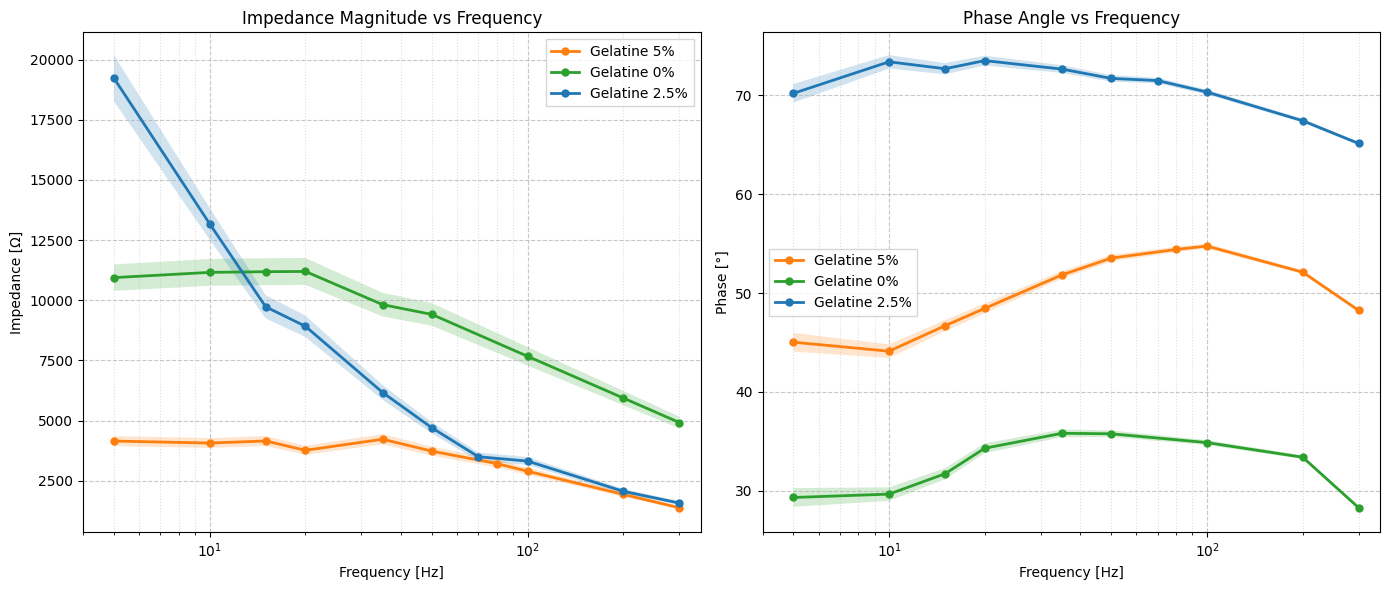
\includegraphics[width=\textwidth]{../../02_Images/gelatine_results.png}
    \caption[Impedance Measurements]{Impedance measurement results for gelatine samples with varying NaCl concentrations.}
    \label{fig:gelatine_results}
\end{figure}


\subsubsection{Signal Localization}

After subjecting a gelatine prototype with 5\% NaCl concentration to the effect of two signal sources placed at fixed coordinates with different frequencies (100 and 900 Hz), the recorded signals are presented in Figure~\ref{fig:localization_gelatine}.

\begin{figure}[H]
    \centering
    \begin{subfigure}[t]{0.43\textwidth}
        \centering
        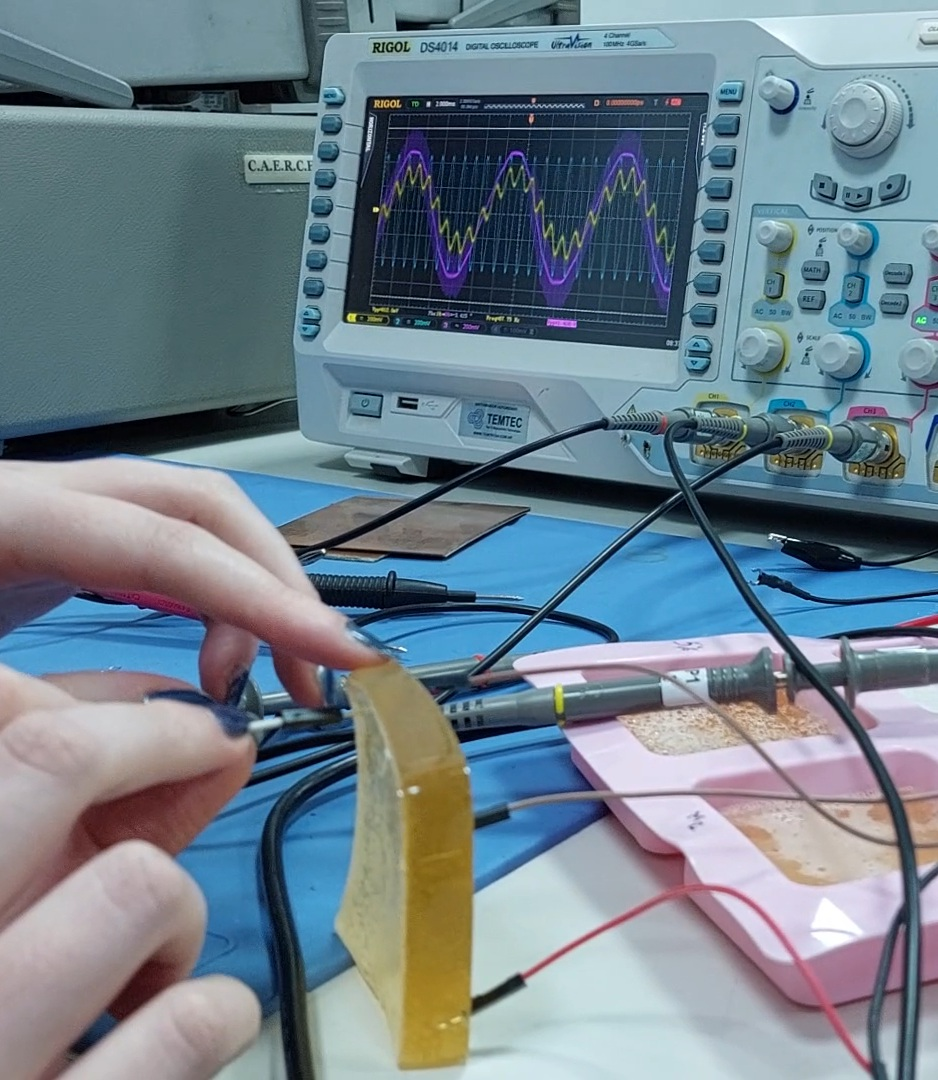
\includegraphics[width=\textwidth]{../../02_Images/near-100-Hz.jpg}
        \caption{Near the 100 Hz source}
        \label{fig:localization_gelatine_100Hz}
    \end{subfigure}
    \hfill
    \begin{subfigure}[t]{0.43\textwidth}
        \centering
        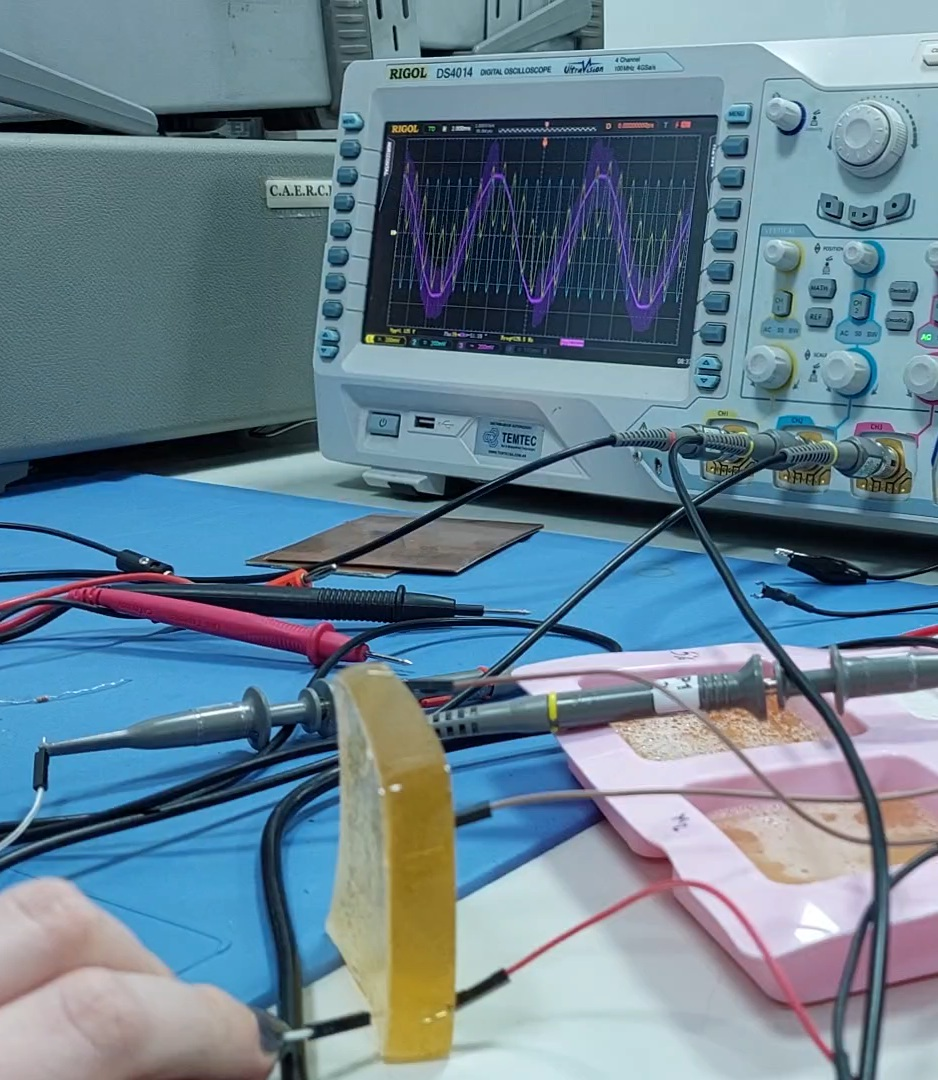
\includegraphics[width=\textwidth]{../../02_Images/near-900-Hz.jpg}
        \caption{Near the 900 Hz source}
        \label{fig:localization_gelatine_900Hz}
    \end{subfigure}
    \caption[Signal Localization]{Signal superposition for gelatine sample with 5\% NaCl concentration subjected to two signal sources with different frequencies.}
    \label{fig:localization_gelatine}
\end{figure}
